The most severe limitation of the survey was undoubtedly in finding respondents. Although the survey was shared on many different social media platforms and developer community pages, it was able to find very few participants compared to the number of people on these platforms and communities. The initial target for the number of participants was 150-200, and a serious effort was made to reach this number.

Besides, some corrections and filtering were made for the 164 responses collected from these Android developers to avoid off-topic responses and collect non-standard answers under a single topic, thus presenting more consistent results both visually and numerically. For example, for some of the questions, there is the option "other" among the answer options offered, and users can choose this option and enter their answers. In this case, when the data is plotted, results such as the following may occur.
\begin{figure}[ht!]
    \centering
    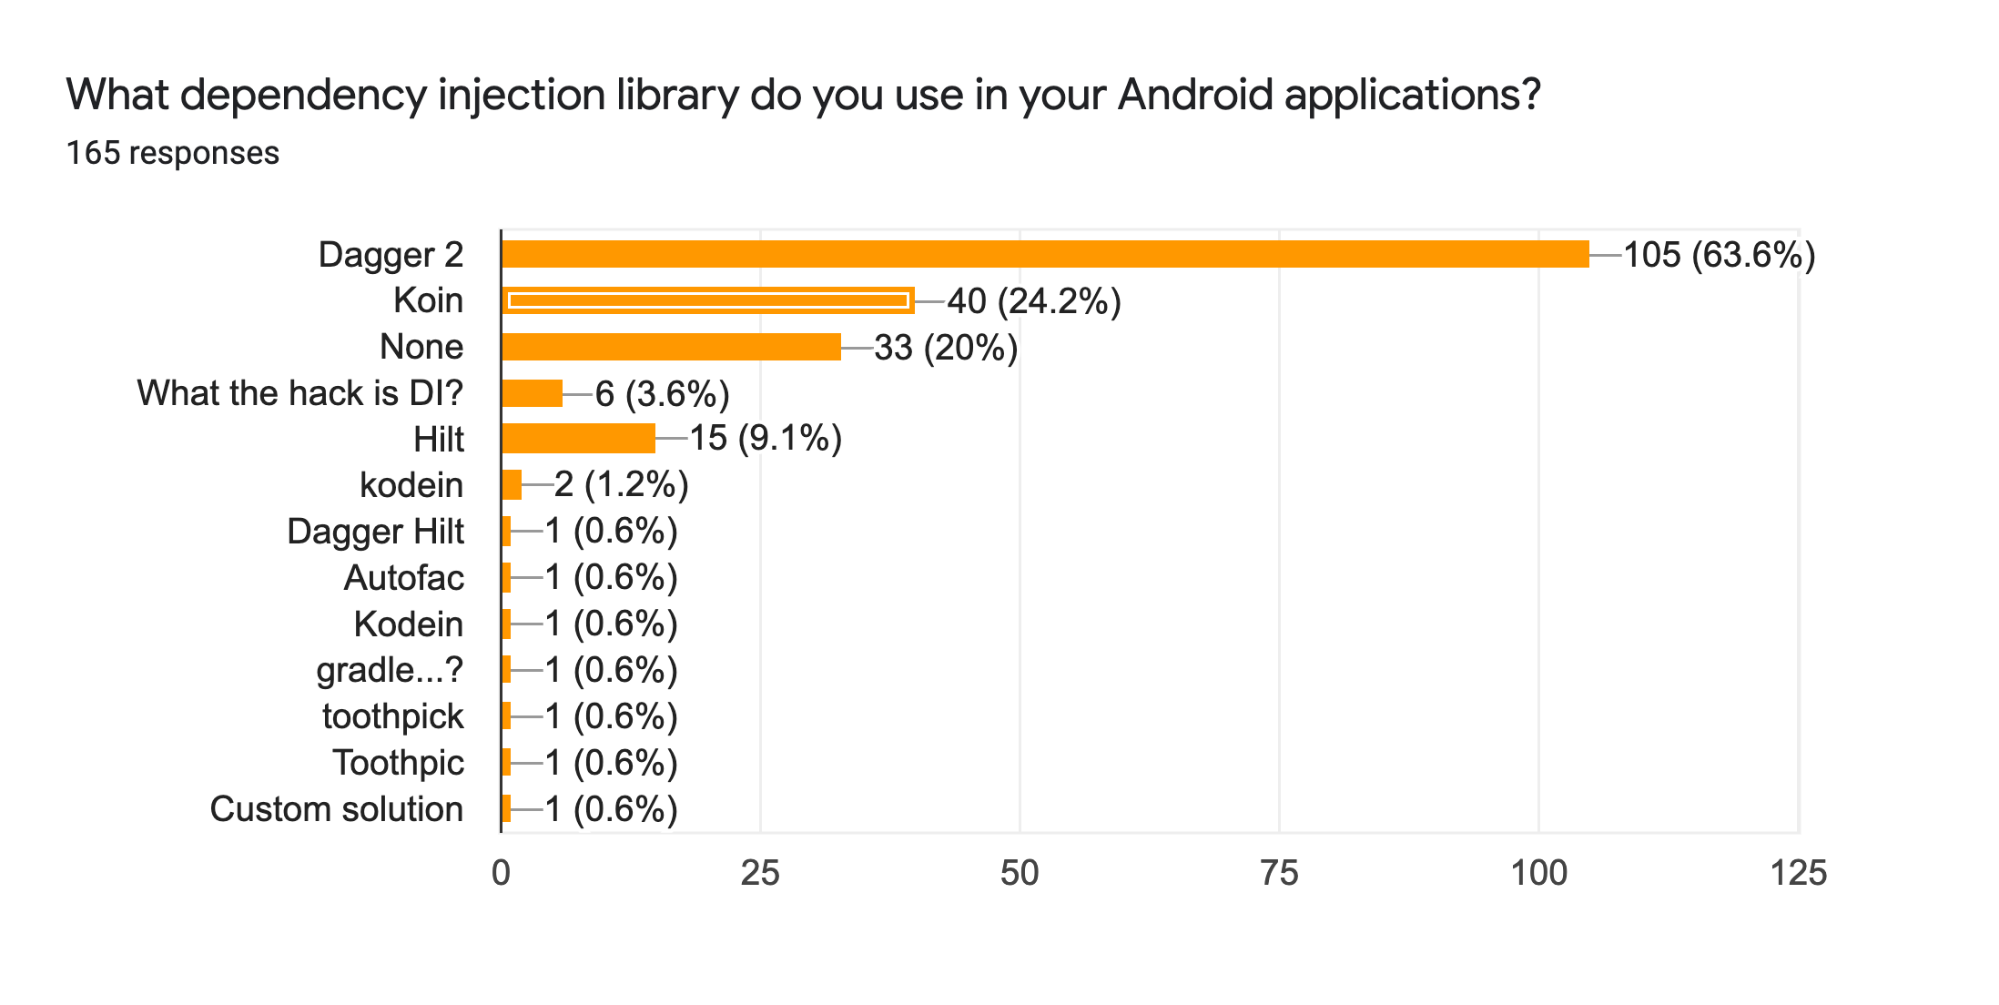
\includegraphics[scale=0.20]{figures/non_standard.png}
    \caption{Example chart plotted with non-standardized answers}
    \label{fig:non_standard_chart_example}
\end{figure}

As shown in the chart, "Toothpick" or “Hilt” libraries do not have a ready-made response option. Android developers using this library have given their answers in different forms. Thus a chart such as this has emerged. Therefore, it was deemed necessary to arrange the inputs in different forms, which correspond to the same answer. 

As an example of the need to filter some answers, a situation in the chart below can be shown. As can be seen in the chart above, which was obtained from the unfiltered survey results, it is seen that developers who develop Android in other forms also participated in the survey. Although it was clearly stated to the participants that the survey included only "Native" Android developers before they filled in the questionnaire, a few such cases were unfortunately not avoided due to the human factor. These kinds of responses have been filtered and edited as they will not contribute to this survey’s purpose and reduce the survey’s accuracy.
\begin{figure}[ht!]
    \centering
    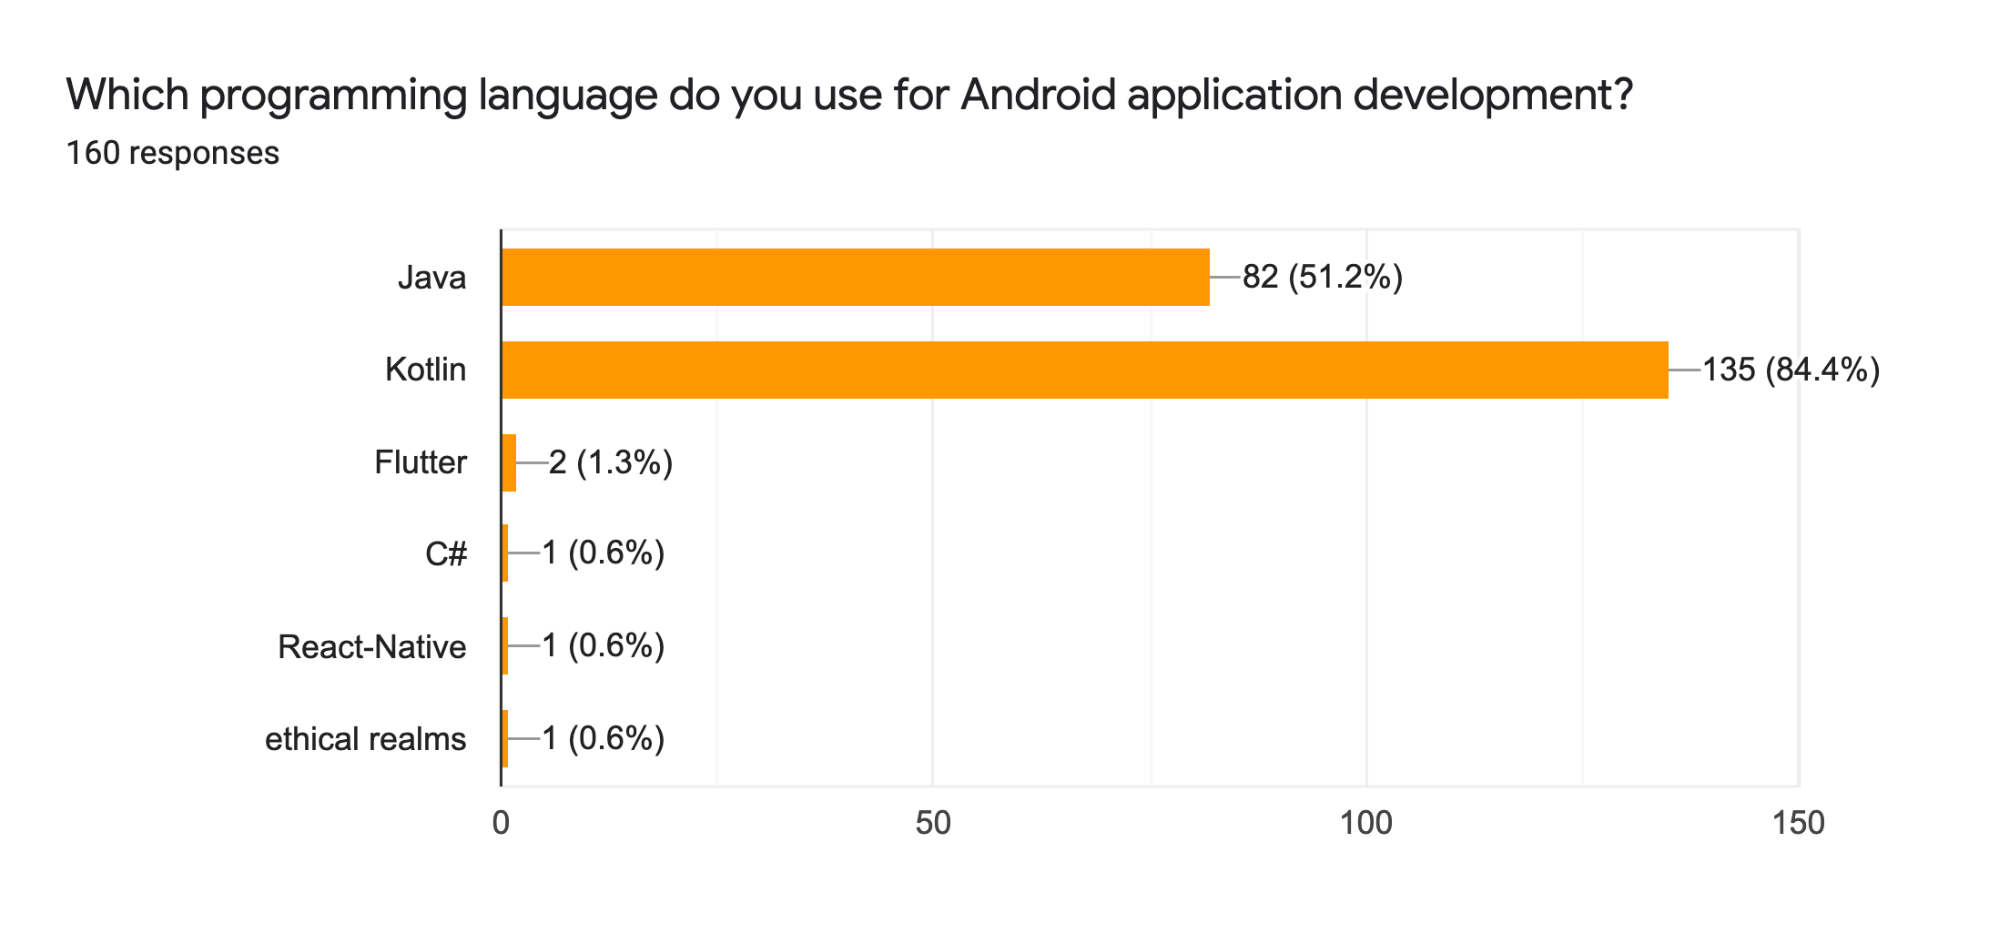
\includegraphics[scale=0.20]{figures/corrupted_chart.png}
    \caption{Example chart plotted with corrupted data}
    \label{fig:corrupted_chart_example}
\end{figure}

The above and other similar situations have been filtered and edited as they will not contribute to the survey's purpose and they reduce the survey’s accuracy. Firstly, the survey results were extracted as a Google Sheets file to do this filtering and editing. Then inappropriate data in this file was corrected or filtered, and finally, the charts and numbers were obtained from the accurate data of the file. While applying corrections and filtering, no changes or manipulations were made on the relevant data. Around 20 of the 164 responses were edited to arrange the inputs in different forms, which correspond to the same answer. Besides, five corrupted responses were removed. After the filtering process, charts were created from the remaining 159 responses to obtain more accurate data. The interpretation of the responses is based on this filtered and corrected final version. The charts obtained through filtered and corrected responses and the data obtained from these charts’ interpretation are presented below, respectively. Since it is possible to choose more than one answer for some questions, it should be taken into account that the total number of answers for each question may exceed the total number of participants. Besides, since the first question was added to the survey a bit later than the answers started being accepted, the answers to these questions are less than the rest. While examining the answers, it will be helpful to consider these two situations to prevent confusion.
